\documentclass[1p]{elsarticle_modified}
%\bibliographystyle{elsarticle-num}

%\usepackage[colorlinks]{hyperref}
%\usepackage{abbrmath_seonhwa} %\Abb, \Ascr, \Acal ,\Abf, \Afrak
\usepackage{amsfonts}
\usepackage{amssymb}
\usepackage{amsmath}
\usepackage{amsthm}
\usepackage{scalefnt}
\usepackage{amsbsy}
\usepackage{kotex}
\usepackage{caption}
\usepackage{subfig}
\usepackage{color}
\usepackage{graphicx}
\usepackage{xcolor} %% white, black, red, green, blue, cyan, magenta, yellow
\usepackage{float}
\usepackage{setspace}
\usepackage{hyperref}

\usepackage{tikz}
\usetikzlibrary{arrows}

\usepackage{multirow}
\usepackage{array} % fixed length table
\usepackage{hhline}

%%%%%%%%%%%%%%%%%%%%%
\makeatletter
\renewcommand*\env@matrix[1][\arraystretch]{%
	\edef\arraystretch{#1}%
	\hskip -\arraycolsep
	\let\@ifnextchar\new@ifnextchar
	\array{*\c@MaxMatrixCols c}}
\makeatother %https://tex.stackexchange.com/questions/14071/how-can-i-increase-the-line-spacing-in-a-matrix
%%%%%%%%%%%%%%%

\usepackage[normalem]{ulem}

\newcommand{\msout}[1]{\ifmmode\text{\sout{\ensuremath{#1}}}\else\sout{#1}\fi}
%SOURCE: \msout is \stkout macro in https://tex.stackexchange.com/questions/20609/strikeout-in-math-mode

\newcommand{\cancel}[1]{
	\ifmmode
	{\color{red}\msout{#1}}
	\else
	{\color{red}\sout{#1}}
	\fi
}

\newcommand{\add}[1]{
	{\color{blue}\uwave{#1}}
}

\newcommand{\replace}[2]{
	\ifmmode
	{\color{red}\msout{#1}}{\color{blue}\uwave{#2}}
	\else
	{\color{red}\sout{#1}}{\color{blue}\uwave{#2}}
	\fi
}

\newcommand{\Sol}{\mathcal{S}} %segment
\newcommand{\D}{D} %diagram
\newcommand{\A}{\mathcal{A}} %arc


%%%%%%%%%%%%%%%%%%%%%%%%%%%%%5 test

\def\sl{\operatorname{\textup{SL}}(2,\Cbb)}
\def\psl{\operatorname{\textup{PSL}}(2,\Cbb)}
\def\quan{\mkern 1mu \triangleright \mkern 1mu}

\theoremstyle{definition}
\newtheorem{thm}{Theorem}[section]
\newtheorem{prop}[thm]{Proposition}
\newtheorem{lem}[thm]{Lemma}
\newtheorem{ques}[thm]{Question}
\newtheorem{cor}[thm]{Corollary}
\newtheorem{defn}[thm]{Definition}
\newtheorem{exam}[thm]{Example}
\newtheorem{rmk}[thm]{Remark}
\newtheorem{alg}[thm]{Algorithm}

\newcommand{\I}{\sqrt{-1}}
\begin{document}

%\begin{frontmatter}
%
%\title{Boundary parabolic representations of knots up to 8 crossings}
%
%%% Group authors per affiliation:
%\author{Yunhi Cho} 
%\address{Department of Mathematics, University of Seoul, Seoul, Korea}
%\ead{yhcho@uos.ac.kr}
%
%
%\author{Seonhwa Kim} %\fnref{s_kim}}
%\address{Center for Geometry and Physics, Institute for Basic Science, Pohang, 37673, Korea}
%\ead{ryeona17@ibs.re.kr}
%
%\author{Hyuk Kim}
%\address{Department of Mathematical Sciences, Seoul National University, Seoul 08826, Korea}
%\ead{hyukkim@snu.ac.kr}
%
%\author{Seokbeom Yoon}
%\address{Department of Mathematical Sciences, Seoul National University, Seoul, 08826,  Korea}
%\ead{sbyoon15@snu.ac.kr}
%
%\begin{abstract}
%We find all boundary parabolic representation of knots up to 8 crossings.
%
%\end{abstract}
%\begin{keyword}
%    \MSC[2010] 57M25 
%\end{keyword}
%
%\end{frontmatter}

%\linenumbers
%\tableofcontents
%
\newcommand\colored[1]{\textcolor{white}{\rule[-0.35ex]{0.8em}{1.4ex}}\kern-0.8em\color{red} #1}%
%\newcommand\colored[1]{\textcolor{white}{ #1}\kern-2.17ex	\textcolor{white}{ #1}\kern-1.81ex	\textcolor{white}{ #1}\kern-2.15ex\color{red}#1	}

{\Large $\underline{11a_{66}~(K11a_{66})}$}

\setlength{\tabcolsep}{10pt}
\renewcommand{\arraystretch}{1.6}
\vspace{1cm}\begin{tabular}{m{100pt}>{\centering\arraybackslash}m{274pt}}
\multirow{5}{120pt}{
	\centering
	\includegraphics[width=112pt]{../../../GIT/diagram.site/Diagrams/png/315_11a_66.png}\\
\ \ \ A knot diagram\footnotemark}&
\allowdisplaybreaks
\textbf{Linearized knot diagam} \\
\cline{2-2}
 &
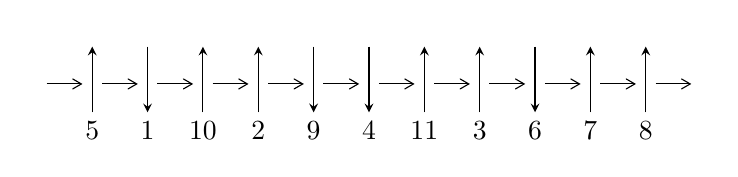
\begin{tikzpicture}[x=20pt, y=17pt]
	% nodes
	\node (C0) at (0, 0) {};
	\node (C1) at (1, 0) {};
	\node (C1U) at (1, +1) {};
	\node (C1D) at (1, -1) {5};

	\node (C2) at (2, 0) {};
	\node (C2U) at (2, +1) {};
	\node (C2D) at (2, -1) {1};

	\node (C3) at (3, 0) {};
	\node (C3U) at (3, +1) {};
	\node (C3D) at (3, -1) {10};

	\node (C4) at (4, 0) {};
	\node (C4U) at (4, +1) {};
	\node (C4D) at (4, -1) {2};

	\node (C5) at (5, 0) {};
	\node (C5U) at (5, +1) {};
	\node (C5D) at (5, -1) {9};

	\node (C6) at (6, 0) {};
	\node (C6U) at (6, +1) {};
	\node (C6D) at (6, -1) {4};

	\node (C7) at (7, 0) {};
	\node (C7U) at (7, +1) {};
	\node (C7D) at (7, -1) {11};

	\node (C8) at (8, 0) {};
	\node (C8U) at (8, +1) {};
	\node (C8D) at (8, -1) {3};

	\node (C9) at (9, 0) {};
	\node (C9U) at (9, +1) {};
	\node (C9D) at (9, -1) {6};

	\node (C10) at (10, 0) {};
	\node (C10U) at (10, +1) {};
	\node (C10D) at (10, -1) {7};

	\node (C11) at (11, 0) {};
	\node (C11U) at (11, +1) {};
	\node (C11D) at (11, -1) {8};
	\node (C12) at (12, 0) {};

	% arrows
	\draw[->,>={angle 60}]
	(C0) edge (C1) (C1) edge (C2) (C2) edge (C3) (C3) edge (C4) (C4) edge (C5) (C5) edge (C6) (C6) edge (C7) (C7) edge (C8) (C8) edge (C9) (C9) edge (C10) (C10) edge (C11) (C11) edge (C12) ;	\draw[->,>=stealth]
	(C1D) edge (C1U) (C2U) edge (C2D) (C3D) edge (C3U) (C4D) edge (C4U) (C5U) edge (C5D) (C6U) edge (C6D) (C7D) edge (C7U) (C8D) edge (C8U) (C9U) edge (C9D) (C10D) edge (C10U) (C11D) edge (C11U) ;
	\end{tikzpicture} \\
\hhline{~~} \\& 
\textbf{Solving Sequence} \\ \cline{2-2} 
 &
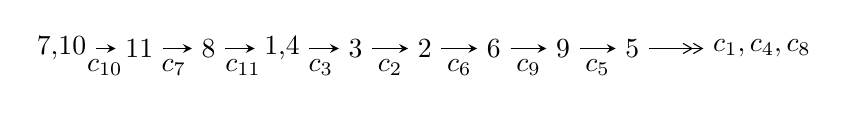
\begin{tikzpicture}[x=25pt, y=7pt]
	% node
	\node (A0) at (-1/8, 0) {7,10};
	\node (A1) at (1, 0) {11};
	\node (A2) at (2, 0) {8};
	\node (A3) at (49/16, 0) {1,4};
	\node (A4) at (33/8, 0) {3};
	\node (A5) at (41/8, 0) {2};
	\node (A6) at (49/8, 0) {6};
	\node (A7) at (57/8, 0) {9};
	\node (A8) at (65/8, 0) {5};
	\node (C1) at (1/2, -1) {$c_{10}$};
	\node (C2) at (3/2, -1) {$c_{7}$};
	\node (C3) at (5/2, -1) {$c_{11}$};
	\node (C4) at (29/8, -1) {$c_{3}$};
	\node (C5) at (37/8, -1) {$c_{2}$};
	\node (C6) at (45/8, -1) {$c_{6}$};
	\node (C7) at (53/8, -1) {$c_{9}$};
	\node (C8) at (61/8, -1) {$c_{5}$};
	\node (A9) at (10, 0) {$c_{1},c_{4},c_{8}$};

	% edge
	\draw[->,>=stealth]	
	(A0) edge (A1) (A1) edge (A2) (A2) edge (A3) (A3) edge (A4) (A4) edge (A5) (A5) edge (A6) (A6) edge (A7) (A7) edge (A8) ;
	\draw[->>,>={angle 60}]	
	(A8) edge (A9);
\end{tikzpicture} \\ 

\end{tabular} \\

\footnotetext{
The image of knot diagram is generated by the software ``\textbf{Draw programme}" developed by Andrew Bartholomew(\url{http://www.layer8.co.uk/maths/draw/index.htm\#Running-draw}), where we modified some parts for our purpose(\url{https://github.com/CATsTAILs/LinksPainter}).
}\phantom \\ \newline 
\centering \textbf{Ideals for irreducible components\footnotemark of $X_{\text{par}}$} 
 
\begin{align*}
I^u_{1}&=\langle 
4.83591\times10^{64} u^{58}-1.44015\times10^{65} u^{57}+\cdots+2.71331\times10^{65} b+7.55669\times10^{64},\\
\phantom{I^u_{1}}&\phantom{= \langle  }-4.47446\times10^{63} u^{58}+4.62488\times10^{64} u^{57}+\cdots+2.71331\times10^{65} a+7.20796\times10^{65},\;u^{59}-5 u^{58}+\cdots+5 u^2-1\rangle \\
\\
\end{align*}
\raggedright * 1 irreducible components of $\dim_{\mathbb{C}}=0$, with total 59 representations.\\
\footnotetext{All coefficients of polynomials are rational numbers. But the coefficients are sometimes approximated in decimal forms when there is not enough margin.}
\newpage
\renewcommand{\arraystretch}{1}
\centering \section*{I. $I^u_{1}= \langle 4.84\times10^{64} u^{58}-1.44\times10^{65} u^{57}+\cdots+2.71\times10^{65} b+7.56\times10^{64},\;-4.47\times10^{63} u^{58}+4.62\times10^{64} u^{57}+\cdots+2.71\times10^{65} a+7.21\times10^{65},\;u^{59}-5 u^{58}+\cdots+5 u^2-1 \rangle$}
\flushleft \textbf{(i) Arc colorings}\\
\begin{tabular}{m{7pt} m{180pt} m{7pt} m{180pt} }
\flushright $a_{7}=$&$\begin{pmatrix}0\\u\end{pmatrix}$ \\
\flushright $a_{10}=$&$\begin{pmatrix}1\\0\end{pmatrix}$ \\
\flushright $a_{11}=$&$\begin{pmatrix}1\\- u^2\end{pmatrix}$ \\
\flushright $a_{8}=$&$\begin{pmatrix}u\\- u^3+u\end{pmatrix}$ \\
\flushright $a_{1}=$&$\begin{pmatrix}- u^2+1\\u^4-2 u^2\end{pmatrix}$ \\
\flushright $a_{4}=$&$\begin{pmatrix}0.0164908 u^{58}-0.170452 u^{57}+\cdots-2.08113 u-2.65652\\-0.178229 u^{58}+0.530775 u^{57}+\cdots+0.638738 u-0.278505\end{pmatrix}$ \\
\flushright $a_{3}=$&$\begin{pmatrix}0.194720 u^{58}-0.701226 u^{57}+\cdots-2.71987 u-2.37802\\-0.178229 u^{58}+0.530775 u^{57}+\cdots+0.638738 u-0.278505\end{pmatrix}$ \\
\flushright $a_{2}=$&$\begin{pmatrix}0.00985244 u^{58}-0.352681 u^{57}+\cdots-2.73901 u-3.24048\\-0.0389600 u^{58}+0.0920662 u^{57}+\cdots+0.321451 u-0.113177\end{pmatrix}$ \\
\flushright $a_{6}=$&$\begin{pmatrix}2.78334 u^{58}-11.1287 u^{57}+\cdots-2.34565 u+5.60971\\0.818170 u^{58}-2.82973 u^{57}+\cdots-0.893777 u+0.202220\end{pmatrix}$ \\
\flushright $a_{9}=$&$\begin{pmatrix}1.33059 u^{58}-7.98023 u^{57}+\cdots+2.66373 u+4.38104\\-0.671853 u^{58}+2.30116 u^{57}+\cdots-1.18700 u-0.702689\end{pmatrix}$ \\
\flushright $a_{5}=$&$\begin{pmatrix}1.35895 u^{58}-4.91224 u^{57}+\cdots-7.98808 u+0.456873\\- u^4+2 u^2\end{pmatrix}$\\ \flushright $a_{5}=$&$\begin{pmatrix}1.35895 u^{58}-4.91224 u^{57}+\cdots-7.98808 u+0.456873\\- u^4+2 u^2\end{pmatrix}$\\&\end{tabular}
\flushleft \textbf{(ii) Obstruction class $= -1$}\\~\\
\flushleft \textbf{(iii) Cusp Shapes $= -3.13284 u^{58}+8.55288 u^{57}+\cdots-6.92957 u+2.03395$}\\~\\
\newpage\renewcommand{\arraystretch}{1}
\flushleft \textbf{(iv) u-Polynomials at the component}\newline \\
\begin{tabular}{m{50pt}|m{274pt}}
Crossings & \hspace{64pt}u-Polynomials at each crossing \\
\hline $$\begin{aligned}c_{1},c_{4}\end{aligned}$$&$\begin{aligned}
&u^{59}+u^{58}+\cdots+14 u-1
\end{aligned}$\\
\hline $$\begin{aligned}c_{2}\end{aligned}$$&$\begin{aligned}
&u^{59}+23 u^{58}+\cdots+198 u-1
\end{aligned}$\\
\hline $$\begin{aligned}c_{3}\end{aligned}$$&$\begin{aligned}
&u^{59}-3 u^{58}+\cdots-4 u+1
\end{aligned}$\\
\hline $$\begin{aligned}c_{5},c_{9}\end{aligned}$$&$\begin{aligned}
&u^{59}+u^{58}+\cdots+5 u^2-1
\end{aligned}$\\
\hline $$\begin{aligned}c_{6}\end{aligned}$$&$\begin{aligned}
&u^{59}+11 u^{58}+\cdots+286 u^2+8
\end{aligned}$\\
\hline $$\begin{aligned}c_{7},c_{10},c_{11}\end{aligned}$$&$\begin{aligned}
&u^{59}-5 u^{58}+\cdots+5 u^2-1
\end{aligned}$\\
\hline $$\begin{aligned}c_{8}\end{aligned}$$&$\begin{aligned}
&u^{59}-15 u^{58}+\cdots-256 u-256
\end{aligned}$\\
\hline
\end{tabular}\\~\\
\newpage\renewcommand{\arraystretch}{1}
\flushleft \textbf{(v) Riley Polynomials at the component}\newline \\
\begin{tabular}{m{50pt}|m{274pt}}
Crossings & \hspace{64pt}Riley Polynomials at each crossing \\
\hline $$\begin{aligned}c_{1},c_{4}\end{aligned}$$&$\begin{aligned}
&y^{59}+23 y^{58}+\cdots+198 y-1
\end{aligned}$\\
\hline $$\begin{aligned}c_{2}\end{aligned}$$&$\begin{aligned}
&y^{59}+27 y^{58}+\cdots+45406 y-1
\end{aligned}$\\
\hline $$\begin{aligned}c_{3}\end{aligned}$$&$\begin{aligned}
&y^{59}-5 y^{58}+\cdots-18 y-1
\end{aligned}$\\
\hline $$\begin{aligned}c_{5},c_{9}\end{aligned}$$&$\begin{aligned}
&y^{59}-37 y^{58}+\cdots+10 y-1
\end{aligned}$\\
\hline $$\begin{aligned}c_{6}\end{aligned}$$&$\begin{aligned}
&y^{59}+279 y^{58}+\cdots-4576 y-64
\end{aligned}$\\
\hline $$\begin{aligned}c_{7},c_{10},c_{11}\end{aligned}$$&$\begin{aligned}
&y^{59}-61 y^{58}+\cdots+10 y-1
\end{aligned}$\\
\hline $$\begin{aligned}c_{8}\end{aligned}$$&$\begin{aligned}
&y^{59}+287 y^{58}+\cdots+1015808 y-65536
\end{aligned}$\\
\hline
\end{tabular}\\~\\
\newpage\flushleft \textbf{(vi) Complex Volumes and Cusp Shapes}
$$\begin{array}{c|c|c}  
\text{Solutions to }I^u_{1}& \I (\text{vol} + \sqrt{-1}CS) & \text{Cusp shape}\\
 \hline 
\begin{aligned}
u &= -0.602290 + 0.803555 I \\
a &= -0.12280 + 1.44745 I \\
b &= -0.907835 + 1.001240 I\end{aligned}
 & -2.44624 - 11.82370 I & \phantom{-0.000000 -}0. + 9.37680 I \\ \hline\begin{aligned}
u &= -0.602290 - 0.803555 I \\
a &= -0.12280 - 1.44745 I \\
b &= -0.907835 - 1.001240 I\end{aligned}
 & -2.44624 + 11.82370 I & \phantom{-0.000000 } 0. - 9.37680 I \\ \hline\begin{aligned}
u &= -0.513328 + 0.905605 I \\
a &= \phantom{-}0.836669 + 0.413786 I \\
b &= \phantom{-}0.607726 + 0.709697 I\end{aligned}
 & -2.77146 + 6.25200 I & \phantom{-0.000000 } 0 \\ \hline\begin{aligned}
u &= -0.513328 - 0.905605 I \\
a &= \phantom{-}0.836669 - 0.413786 I \\
b &= \phantom{-}0.607726 - 0.709697 I\end{aligned}
 & -2.77146 - 6.25200 I & \phantom{-0.000000 } 0 \\ \hline\begin{aligned}
u &= \phantom{-}0.780237 + 0.719781 I \\
a &= \phantom{-}0.262671 + 0.669150 I \\
b &= \phantom{-}0.668932 + 0.384075 I\end{aligned}
 & \phantom{-}2.44555 + 0.67895 I & \phantom{-0.000000 } 0 \\ \hline\begin{aligned}
u &= \phantom{-}0.780237 - 0.719781 I \\
a &= \phantom{-}0.262671 - 0.669150 I \\
b &= \phantom{-}0.668932 - 0.384075 I\end{aligned}
 & \phantom{-}2.44555 - 0.67895 I & \phantom{-0.000000 } 0 \\ \hline\begin{aligned}
u &= -0.610415 + 0.675553 I \\
a &= \phantom{-}0.09095 - 1.51512 I \\
b &= \phantom{-}0.869792 - 1.011370 I\end{aligned}
 & -0.53563 - 6.33799 I & \phantom{-}3.85891 + 5.79197 I \\ \hline\begin{aligned}
u &= -0.610415 - 0.675553 I \\
a &= \phantom{-}0.09095 + 1.51512 I \\
b &= \phantom{-}0.869792 + 1.011370 I\end{aligned}
 & -0.53563 + 6.33799 I & \phantom{-}3.85891 - 5.79197 I \\ \hline\begin{aligned}
u &= -0.738862 + 0.507440 I \\
a &= \phantom{-}0.784790 - 0.069867 I \\
b &= \phantom{-}0.451996 + 0.888554 I\end{aligned}
 & -5.18481 + 0.07298 I & -2.77397 + 1.06751 I \\ \hline\begin{aligned}
u &= -0.738862 - 0.507440 I \\
a &= \phantom{-}0.784790 + 0.069867 I \\
b &= \phantom{-}0.451996 - 0.888554 I\end{aligned}
 & -5.18481 - 0.07298 I & -2.77397 - 1.06751 I\\
 \hline 
 \end{array}$$\newpage$$\begin{array}{c|c|c}  
\text{Solutions to }I^u_{1}& \I (\text{vol} + \sqrt{-1}CS) & \text{Cusp shape}\\
 \hline 
\begin{aligned}
u &= \phantom{-}0.610635 + 0.920920 I \\
a &= -0.371965 - 0.691396 I \\
b &= -0.678927 - 0.415007 I\end{aligned}
 & \phantom{-}1.69330 + 5.46743 I & \phantom{-0.000000 } 0 \\ \hline\begin{aligned}
u &= \phantom{-}0.610635 - 0.920920 I \\
a &= -0.371965 + 0.691396 I \\
b &= -0.678927 + 0.415007 I\end{aligned}
 & \phantom{-}1.69330 - 5.46743 I & \phantom{-0.000000 } 0 \\ \hline\begin{aligned}
u &= \phantom{-}1.179590 + 0.072832 I \\
a &= \phantom{-}0.023949 + 0.735583 I \\
b &= \phantom{-}0.504296 + 0.524843 I\end{aligned}
 & \phantom{-}1.93352 - 0.03829 I & \phantom{-0.000000 } 0 \\ \hline\begin{aligned}
u &= \phantom{-}1.179590 - 0.072832 I \\
a &= \phantom{-}0.023949 - 0.735583 I \\
b &= \phantom{-}0.504296 - 0.524843 I\end{aligned}
 & \phantom{-}1.93352 + 0.03829 I & \phantom{-0.000000 } 0 \\ \hline\begin{aligned}
u &= -0.298346 + 0.756487 I \\
a &= -1.040070 - 0.594848 I \\
b &= -0.539223 - 0.629121 I\end{aligned}
 & -1.35810 + 1.65554 I & \phantom{-}2.46202 - 2.77708 I \\ \hline\begin{aligned}
u &= -0.298346 - 0.756487 I \\
a &= -1.040070 + 0.594848 I \\
b &= -0.539223 + 0.629121 I\end{aligned}
 & -1.35810 - 1.65554 I & \phantom{-}2.46202 + 2.77708 I \\ \hline\begin{aligned}
u &= -0.331322 + 0.631890 I \\
a &= -0.28163 + 1.56746 I \\
b &= -0.92852 + 1.10882 I\end{aligned}
 & -6.37379 - 4.04787 I & -3.93072 + 5.51814 I \\ \hline\begin{aligned}
u &= -0.331322 - 0.631890 I \\
a &= -0.28163 - 1.56746 I \\
b &= -0.92852 - 1.10882 I\end{aligned}
 & -6.37379 + 4.04787 I & -3.93072 - 5.51814 I \\ \hline\begin{aligned}
u &= -1.384970 + 0.131008 I \\
a &= -0.737163 - 0.719110 I \\
b &= \phantom{-}1.026640 - 0.458872 I\end{aligned}
 & \phantom{-}3.26189 - 3.67751 I & \phantom{-0.000000 } 0 \\ \hline\begin{aligned}
u &= -1.384970 - 0.131008 I \\
a &= -0.737163 + 0.719110 I \\
b &= \phantom{-}1.026640 + 0.458872 I\end{aligned}
 & \phantom{-}3.26189 + 3.67751 I & \phantom{-0.000000 } 0\\
 \hline 
 \end{array}$$\newpage$$\begin{array}{c|c|c}  
\text{Solutions to }I^u_{1}& \I (\text{vol} + \sqrt{-1}CS) & \text{Cusp shape}\\
 \hline 
\begin{aligned}
u &= -1.42247 + 0.01167 I \\
a &= -4.44893 + 9.36868 I \\
b &= \phantom{-}0.072559 + 0.149112 I\end{aligned}
 & \phantom{-}3.30587 - 2.05347 I & \phantom{-0.000000 } 0 \\ \hline\begin{aligned}
u &= -1.42247 - 0.01167 I \\
a &= -4.44893 - 9.36868 I \\
b &= \phantom{-}0.072559 - 0.149112 I\end{aligned}
 & \phantom{-}3.30587 + 2.05347 I & \phantom{-0.000000 } 0 \\ \hline\begin{aligned}
u &= \phantom{-}0.009641 + 0.561258 I \\
a &= -0.84390 - 1.40804 I \\
b &= -0.499557 - 0.473604 I\end{aligned}
 & -1.27830 + 1.37033 I & -1.75929 - 4.49534 I \\ \hline\begin{aligned}
u &= \phantom{-}0.009641 - 0.561258 I \\
a &= -0.84390 + 1.40804 I \\
b &= -0.499557 + 0.473604 I\end{aligned}
 & -1.27830 - 1.37033 I & -1.75929 + 4.49534 I \\ \hline\begin{aligned}
u &= \phantom{-}1.43879 + 0.18099 I \\
a &= -0.623609 + 0.710901 I \\
b &= \phantom{-}1.51759 + 1.20583 I\end{aligned}
 & -0.67928 + 6.89950 I & \phantom{-0.000000 } 0 \\ \hline\begin{aligned}
u &= \phantom{-}1.43879 - 0.18099 I \\
a &= -0.623609 - 0.710901 I \\
b &= \phantom{-}1.51759 - 1.20583 I\end{aligned}
 & -0.67928 - 6.89950 I & \phantom{-0.000000 } 0 \\ \hline\begin{aligned}
u &= \phantom{-}1.45449\phantom{ +0.000000I} \\
a &= \phantom{-}0.915660\phantom{ +0.000000I} \\
b &= -0.262354\phantom{ +0.000000I}\end{aligned}
 & \phantom{-}3.37740\phantom{ +0.000000I} & \phantom{-0.000000 } 0 \\ \hline\begin{aligned}
u &= \phantom{-}0.402436 + 0.343152 I \\
a &= -0.669541 + 0.915825 I \\
b &= -1.23192 + 0.73590 I\end{aligned}
 & -1.56344 + 4.78630 I & \phantom{-}2.02963 - 10.35215 I \\ \hline\begin{aligned}
u &= \phantom{-}0.402436 - 0.343152 I \\
a &= -0.669541 - 0.915825 I \\
b &= -1.23192 - 0.73590 I\end{aligned}
 & -1.56344 - 4.78630 I & \phantom{-}2.02963 + 10.35215 I \\ \hline\begin{aligned}
u &= \phantom{-}0.526798 + 0.021630 I \\
a &= \phantom{-}0.188140 + 0.404628 I \\
b &= \phantom{-}0.891983 + 0.249450 I\end{aligned}
 & \phantom{-}1.131640 + 0.063901 I & \phantom{-}10.49402 + 0.56940 I\\
 \hline 
 \end{array}$$\newpage$$\begin{array}{c|c|c}  
\text{Solutions to }I^u_{1}& \I (\text{vol} + \sqrt{-1}CS) & \text{Cusp shape}\\
 \hline 
\begin{aligned}
u &= \phantom{-}0.526798 - 0.021630 I \\
a &= \phantom{-}0.188140 - 0.404628 I \\
b &= \phantom{-}0.891983 - 0.249450 I\end{aligned}
 & \phantom{-}1.131640 - 0.063901 I & \phantom{-}10.49402 - 0.56940 I \\ \hline\begin{aligned}
u &= \phantom{-}1.47328 + 0.05201 I \\
a &= -0.062797 - 0.841379 I \\
b &= \phantom{-}0.39778 - 1.37113 I\end{aligned}
 & \phantom{-}6.50993 + 3.19293 I & \phantom{-0.000000 } 0 \\ \hline\begin{aligned}
u &= \phantom{-}1.47328 - 0.05201 I \\
a &= -0.062797 + 0.841379 I \\
b &= \phantom{-}0.39778 + 1.37113 I\end{aligned}
 & \phantom{-}6.50993 - 3.19293 I & \phantom{-0.000000 } 0 \\ \hline\begin{aligned}
u &= -1.47786 + 0.08730 I \\
a &= -0.045066 + 0.186936 I \\
b &= \phantom{-}1.71673 + 1.40690 I\end{aligned}
 & \phantom{-}4.61526 - 6.26348 I & \phantom{-0.000000 } 0 \\ \hline\begin{aligned}
u &= -1.47786 - 0.08730 I \\
a &= -0.045066 - 0.186936 I \\
b &= \phantom{-}1.71673 - 1.40690 I\end{aligned}
 & \phantom{-}4.61526 + 6.26348 I & \phantom{-0.000000 } 0 \\ \hline\begin{aligned}
u &= -0.490640 + 0.130399 I \\
a &= -0.01807 - 2.09045 I \\
b &= \phantom{-}0.412044 - 1.147950 I\end{aligned}
 & \phantom{-}0.68155 - 2.84567 I & \phantom{-}8.20760 + 7.93876 I \\ \hline\begin{aligned}
u &= -0.490640 - 0.130399 I \\
a &= -0.01807 + 2.09045 I \\
b &= \phantom{-}0.412044 + 1.147950 I\end{aligned}
 & \phantom{-}0.68155 + 2.84567 I & \phantom{-}8.20760 - 7.93876 I \\ \hline\begin{aligned}
u &= \phantom{-}1.49940 + 0.03329 I \\
a &= \phantom{-}0.219999 - 0.701654 I \\
b &= -0.91452 - 1.88246 I\end{aligned}
 & \phantom{-}7.24513 + 3.41415 I & \phantom{-0.000000 } 0 \\ \hline\begin{aligned}
u &= \phantom{-}1.49940 - 0.03329 I \\
a &= \phantom{-}0.219999 + 0.701654 I \\
b &= -0.91452 + 1.88246 I\end{aligned}
 & \phantom{-}7.24513 - 3.41415 I & \phantom{-0.000000 } 0 \\ \hline\begin{aligned}
u &= -1.50177 + 0.00830 I \\
a &= \phantom{-}0.297564 + 0.231736 I \\
b &= -1.67755 + 0.55669 I\end{aligned}
 & \phantom{-}7.78177 - 0.18045 I & \phantom{-0.000000 } 0\\
 \hline 
 \end{array}$$\newpage$$\begin{array}{c|c|c}  
\text{Solutions to }I^u_{1}& \I (\text{vol} + \sqrt{-1}CS) & \text{Cusp shape}\\
 \hline 
\begin{aligned}
u &= -1.50177 - 0.00830 I \\
a &= \phantom{-}0.297564 - 0.231736 I \\
b &= -1.67755 - 0.55669 I\end{aligned}
 & \phantom{-}7.78177 + 0.18045 I & \phantom{-0.000000 } 0 \\ \hline\begin{aligned}
u &= \phantom{-}1.55701 + 0.22591 I \\
a &= \phantom{-}0.536066 - 0.912338 I \\
b &= -1.21260 - 1.20134 I\end{aligned}
 & \phantom{-}6.60505 + 9.68161 I & \phantom{-0.000000 } 0 \\ \hline\begin{aligned}
u &= \phantom{-}1.55701 - 0.22591 I \\
a &= \phantom{-}0.536066 + 0.912338 I \\
b &= -1.21260 + 1.20134 I\end{aligned}
 & \phantom{-}6.60505 - 9.68161 I & \phantom{-0.000000 } 0 \\ \hline\begin{aligned}
u &= \phantom{-}1.56490 + 0.27474 I \\
a &= -0.575143 + 0.964495 I \\
b &= \phantom{-}1.19103 + 1.13486 I\end{aligned}
 & \phantom{-}4.6425 + 15.8011 I & \phantom{-0.000000 } 0 \\ \hline\begin{aligned}
u &= \phantom{-}1.56490 - 0.27474 I \\
a &= -0.575143 - 0.964495 I \\
b &= \phantom{-}1.19103 - 1.13486 I\end{aligned}
 & \phantom{-}4.6425 - 15.8011 I & \phantom{-0.000000 } 0 \\ \hline\begin{aligned}
u &= -1.57947 + 0.22255 I \\
a &= \phantom{-}0.272883 + 0.711732 I \\
b &= -1.148480 + 0.713126 I\end{aligned}
 & \phantom{-}10.09090 - 4.09953 I & \phantom{-0.000000 } 0 \\ \hline\begin{aligned}
u &= -1.57947 - 0.22255 I \\
a &= \phantom{-}0.272883 - 0.711732 I \\
b &= -1.148480 - 0.713126 I\end{aligned}
 & \phantom{-}10.09090 + 4.09953 I & \phantom{-0.000000 } 0 \\ \hline\begin{aligned}
u &= \phantom{-}0.023287 + 0.400883 I \\
a &= -0.56139 - 3.63273 I \\
b &= -0.438386 - 0.419133 I\end{aligned}
 & -1.06640 + 1.39300 I & -4.87303 - 6.40557 I \\ \hline\begin{aligned}
u &= \phantom{-}0.023287 - 0.400883 I \\
a &= -0.56139 + 3.63273 I \\
b &= -0.438386 + 0.419133 I\end{aligned}
 & -1.06640 - 1.39300 I & -4.87303 + 6.40557 I \\ \hline\begin{aligned}
u &= -1.57430 + 0.29595 I \\
a &= -0.251509 - 0.797155 I \\
b &= \phantom{-}1.101890 - 0.732255 I\end{aligned}
 & \phantom{-}8.82124 - 9.84696 I & \phantom{-0.000000 } 0\\
 \hline 
 \end{array}$$\newpage$$\begin{array}{c|c|c}  
\text{Solutions to }I^u_{1}& \I (\text{vol} + \sqrt{-1}CS) & \text{Cusp shape}\\
 \hline 
\begin{aligned}
u &= -1.57430 - 0.29595 I \\
a &= -0.251509 + 0.797155 I \\
b &= \phantom{-}1.101890 + 0.732255 I\end{aligned}
 & \phantom{-}8.82124 + 9.84696 I & \phantom{-0.000000 } 0 \\ \hline\begin{aligned}
u &= -0.344914 + 0.168527 I \\
a &= \phantom{-}0.30650 - 2.60805 I \\
b &= -0.194817 - 0.606555 I\end{aligned}
 & \phantom{-}0.46273 - 2.38122 I & \phantom{-}3.10427 + 1.63624 I \\ \hline\begin{aligned}
u &= -0.344914 - 0.168527 I \\
a &= \phantom{-}0.30650 + 2.60805 I \\
b &= -0.194817 + 0.606555 I\end{aligned}
 & \phantom{-}0.46273 + 2.38122 I & \phantom{-}3.10427 - 1.63624 I \\ \hline\begin{aligned}
u &= \phantom{-}0.253207 + 0.285102 I \\
a &= -3.18179 + 4.75906 I \\
b &= \phantom{-}0.552194 + 0.272160 I\end{aligned}
 & -1.85782 - 2.60565 I & \phantom{-}2.86490 - 11.40100 I \\ \hline\begin{aligned}
u &= \phantom{-}0.253207 - 0.285102 I \\
a &= -3.18179 - 4.75906 I \\
b &= \phantom{-}0.552194 - 0.272160 I\end{aligned}
 & -1.85782 + 2.60565 I & \phantom{-}2.86490 + 11.40100 I \\ \hline\begin{aligned}
u &= \phantom{-}1.61782 + 0.39605 I \\
a &= \phantom{-}0.061041 + 0.323493 I \\
b &= \phantom{-}0.609284 + 0.193792 I\end{aligned}
 & \phantom{-}4.33658 + 3.40939 I & \phantom{-0.000000 } 0 \\ \hline\begin{aligned}
u &= \phantom{-}1.61782 - 0.39605 I \\
a &= \phantom{-}0.061041 - 0.323493 I \\
b &= \phantom{-}0.609284 - 0.193792 I\end{aligned}
 & \phantom{-}4.33658 - 3.40939 I & \phantom{-0.000000 } 0 \\ \hline\begin{aligned}
u &= \phantom{-}1.70668 + 0.24332 I \\
a &= -0.003673 - 0.211471 I \\
b &= -0.588967 - 0.121325 I\end{aligned}
 & \phantom{-}4.61241 - 1.25946 I & \phantom{-0.000000 } 0 \\ \hline\begin{aligned}
u &= \phantom{-}1.70668 - 0.24332 I \\
a &= -0.003673 + 0.211471 I \\
b &= -0.588967 + 0.121325 I\end{aligned}
 & \phantom{-}4.61241 + 1.25946 I & \phantom{-0.000000 } 0\\
 \hline 
 \end{array}$$\newpage
\newpage\renewcommand{\arraystretch}{1}
\centering \section*{ II. u-Polynomials}
\begin{tabular}{m{50pt}|m{274pt}}
Crossings & \hspace{64pt}u-Polynomials at each crossing \\
\hline $$\begin{aligned}c_{1},c_{4}\end{aligned}$$&$\begin{aligned}
&u^{59}+u^{58}+\cdots+14 u-1
\end{aligned}$\\
\hline $$\begin{aligned}c_{2}\end{aligned}$$&$\begin{aligned}
&u^{59}+23 u^{58}+\cdots+198 u-1
\end{aligned}$\\
\hline $$\begin{aligned}c_{3}\end{aligned}$$&$\begin{aligned}
&u^{59}-3 u^{58}+\cdots-4 u+1
\end{aligned}$\\
\hline $$\begin{aligned}c_{5},c_{9}\end{aligned}$$&$\begin{aligned}
&u^{59}+u^{58}+\cdots+5 u^2-1
\end{aligned}$\\
\hline $$\begin{aligned}c_{6}\end{aligned}$$&$\begin{aligned}
&u^{59}+11 u^{58}+\cdots+286 u^2+8
\end{aligned}$\\
\hline $$\begin{aligned}c_{7},c_{10},c_{11}\end{aligned}$$&$\begin{aligned}
&u^{59}-5 u^{58}+\cdots+5 u^2-1
\end{aligned}$\\
\hline $$\begin{aligned}c_{8}\end{aligned}$$&$\begin{aligned}
&u^{59}-15 u^{58}+\cdots-256 u-256
\end{aligned}$\\
\hline
\end{tabular}\newpage\renewcommand{\arraystretch}{1}
\centering \section*{ III. Riley Polynomials}
\begin{tabular}{m{50pt}|m{274pt}}
Crossings & \hspace{64pt}Riley Polynomials at each crossing \\
\hline $$\begin{aligned}c_{1},c_{4}\end{aligned}$$&$\begin{aligned}
&y^{59}+23 y^{58}+\cdots+198 y-1
\end{aligned}$\\
\hline $$\begin{aligned}c_{2}\end{aligned}$$&$\begin{aligned}
&y^{59}+27 y^{58}+\cdots+45406 y-1
\end{aligned}$\\
\hline $$\begin{aligned}c_{3}\end{aligned}$$&$\begin{aligned}
&y^{59}-5 y^{58}+\cdots-18 y-1
\end{aligned}$\\
\hline $$\begin{aligned}c_{5},c_{9}\end{aligned}$$&$\begin{aligned}
&y^{59}-37 y^{58}+\cdots+10 y-1
\end{aligned}$\\
\hline $$\begin{aligned}c_{6}\end{aligned}$$&$\begin{aligned}
&y^{59}+279 y^{58}+\cdots-4576 y-64
\end{aligned}$\\
\hline $$\begin{aligned}c_{7},c_{10},c_{11}\end{aligned}$$&$\begin{aligned}
&y^{59}-61 y^{58}+\cdots+10 y-1
\end{aligned}$\\
\hline $$\begin{aligned}c_{8}\end{aligned}$$&$\begin{aligned}
&y^{59}+287 y^{58}+\cdots+1015808 y-65536
\end{aligned}$\\
\hline
\end{tabular}
\vskip 2pc
\end{document}